\section{CTST - Lớp 10 - Ôn tập giữa học kì 1 - Đề 3}

\caulc

\Opensolutionfile{ans}[ans-ABCD]

\begin{ex}%[0D1H1-2]%[CTST - Lớp 10 - Ôn tập giữa học kì 1 - Đề 3]%[Nguyễn Hoài Nam]
	Trong các mệnh đề sau, mệnh đề nào là mệnh đề \textbf{sai}?
	\choice
	{\True $\forall x\in \mathbb{R}: x^2>0$}
	{$\exists x\in \mathbb{R}: x>x^2$}
	{$\exists n\in \mathbb{N}: n^2=n$}
	{$\forall n\in \mathbb{N}: n^2>0$}
	\loigiai{
		Ta có $0\in\mathbb{R}$ và $0^2=0$ nên mệnh đề $\forall x\in \mathbb{R}: x^2>0$ là mệnh đề sai.
	}
	
	
\end{ex}

\begin{ex}%[0D1N2-1]%[CTST - Lớp 10 - Ôn tập giữa học kì 1 - Đề 3]%[Nguyễn Hoài Nam]
	Cho tập hợp $A$. Trong các mệnh đề sau đây, mệnh đề nào \textbf{sai}?
	\choice
	{$A\subset A$}
	{$\varnothing \subset A$}
	{\True $A\in\varnothing $}
	{$\varnothing  \subset \varnothing $}
	\loigiai{Do $A$ là một tập hợp nên mệnh đề  $A\in \varnothing $ là mệnh đề sai.}
\end{ex}

\begin{ex}%[0D2N1-2]%[CTST - Lớp 10 - Ôn tập giữa học kì 1 - Đề 3]%[Nguyễn Hoài Nam]
	Điểm $A(-1;3)$ là điểm thuộc miền nghiệm của bất phương trình
	\choice
	{\True $-3x+2y-4>0$}
	{$x+3y+1<0$}
	{$3x-y-2>0$}
	{$2x-y+4>0$}
	\loigiai{Vì $-3\cdot (-1)+2\cdot 3-4>0$ là mệnh đề đúng nên $A(-1;3)$ là điểm thuộc miền nghiệm của bất phương trình $-3x+2y-4>0$.}
\end{ex}

\begin{ex}%[0D3H1-2]%[CTST - Lớp 10 - Ôn tập giữa học kì 1 - Đề 3]%[Nguyễn Hoài Nam]
	Hàm số $y=f(x)=\sqrt{x+1}+\dfrac{1}{x^2-4}$ có tập xác định là $\mathscr{D}$ là
	\choice
	{$\mathscr{D}=[-1;+\infty)$}
	{$\mathscr{D}=\mathbb{R}\setminus\{-2;2\}$}
	{\True $\mathscr{D}=[-1;+\infty)\setminus \{2\}$}
	{$\mathscr{D}=[2;+\infty)$}
	\loigiai{Hàm số đã cho xác định khi và chỉ khi $\heva{&x+1\ge 0\\&x^2-4\ne 0}\Leftrightarrow \heva{&x\ge -1\\&x\ne \pm 2}\Leftrightarrow x\in[-1;+\infty)\setminus\{2\}$.\\
		Vậy hàm số đã cho có tập xác định là $\mathscr{D}=[-1;+\infty)\setminus \{2\}$. }
\end{ex}


\begin{ex}%[0D3H1-2]%[CTST - Lớp 10 - Ôn tập giữa học kì 1 - Đề 3]%[Nguyễn Hoài Nam]
	Để hàm số $y=f(x)=(m-1)(x+2024)^2+(m^2-1)|x-2025|+10$ là một hàm số bậc hai thì giá trị của $m$ là 
	\choice
	{1}{1 hoặc -1}{\True-1}{2025}
	\loigiai{Hàm số đã cho là hàm số bậc hai khi và chỉ khi $\heva{&m-1\ne 0\\&m^2-1=0}\Leftrightarrow\heva{&m\ne 1\\&m=\pm 1}\Leftrightarrow m=-1$.\\
		Vậy để hàm số đã cho là hàm số bậc hai thì $m=-1$.}
\end{ex}

\begin{ex}%[0D1H1-2]%[CTST - Lớp 10 - Ôn tập giữa học kì 1 - Đề 3]%[Nguyễn Hoài Nam]
	Mệnh đề nào đúng trong các mệnh đề sau?
	\choice
	{$P:\exists x,y\in\mathbb{R}: 2x^2+5y^2+2xy<0$}
	{$Q:\exists n \in\mathbb{N}, n^2+1$ chia hết cho $4$}
	{\True $R:\forall n\in\mathbb{Z},\exists m\in\mathbb{N}: m+n\in\mathbb{N}$ }
	{$S:\forall x\in\mathbb{N^*},x+\dfrac{3}{x}\ge 4$}
	\loigiai{
		\begin{enumerate}
			\item[-] 	Xét mệnh đề $P:\exists x,y\in\mathbb{R}: 2x^2+5y^2+2xy<0$.\\
			Do $2x^2+5y^2+2xy=(x+y)^2+x^2+4y^2\ge 0$ nên $P$ là mệnh đề sai.
			\item[-]  Xét mệnh đề $Q:\exists n \in\mathbb{N}, n^2+1$ chia hết cho $4$.\\
			Với bất kì số tự nhiên $n$, ta có
			\begin{enumerate}
				\item[+] Nếu $n=2k\ (k\in\mathbb{N})$ thì $n^2+1=4k^2+1$ không chia hết cho 4.
				\item[+] Nếu $n=2k+1\ (k\in\mathbb{N})$ thì $n^2+1=4k^2+4k+2=4(k^2+k)+2$ không chia hết 4.\\
				Vậy $Q$ là mệnh đề sai.
			\end{enumerate}
			\item[-] Xét mệnh đề $R:\forall n\in\mathbb{Z},\exists m\in\mathbb{N}: m+n\in\mathbb{N}$.\\
			Với mọi số nguyên $n$, ta chọn $m=|n|+1$. Khi đó, $m+n=n+|n|+1$ luôn là số tự nhiên.\\
			Vậy $R$ là mệnh đề đúng.
			\item[-] Với $x=2$ thì $2+\dfrac{3}{2}<4$ nên mệnh đề $S$ là mệnh đề sai.
		\end{enumerate}
	}
\end{ex}
\begin{ex}%[0D1N3-3]%[CTST - Lớp 10 - Ôn tập giữa học kì 1 - Đề 3]%[Nguyễn Hoài Nam]
	Cho hai tập hợp $A=\{x \in \mathbb{R} \mid -5 \le x<1\}$; $B=\{ x\in \mathbb{R} \mid -3 <x \le 3 \}$. Tìm $A \cup B$.
	\choice
	{$[-5;3)$}
	{$(-3;1)$}
	{$(1;3]$}
	{\True $[-5;3]$}
	\loigiai
	{
		Ta có $A=[-5;1)$, $B=(-3;3]$. Vậy $A \cup B = [-5;3]$.
	}
\end{ex}

\begin{ex}%[0D2N2-1]%[CTST - Lớp 10 - Ôn tập giữa học kì 1 - Đề 3]%[Nguyễn Hoài Nam]
	Điểm nào sau đây thuộc miền nghiệm của hệ bất phương trình bậc nhất hai ẩn $\heva{&3x-y<0 \\ & x+y \ge 2}$?
	\choice
	{$(5;1)$}
	{\True $(1;4)$}
	{$(1;1)$}
	{$(0;0)$}
	\loigiai
	{
		Thay tọa độ từng điểm trong các phương án vào hệ bất phương trình đã cho, ta thấy chỉ có $(1;4)$ thỏa mãn vì $\heva{&3\cdot 1 -4<0 \\ & 1+4 \ge 2.}$
	}
\end{ex}

\begin{ex}%[0D3N1-5]%[CTST - Lớp 10 - Ôn tập giữa học kì 1 - Đề 3]%[Nguyễn Hoài Nam]
	\immini{Cho hàm số $y=f(x)$ có đồ thị như hình vẽ. Chọn khẳng định đúng.
		\choice
		{Hàm số nghịch biến trên khoảng $(-2;2)$}
		{\True Hàm số đồng biến trên khoảng $(1;3)$}
		{Đồ thị hàm số đi qua điểm $(2;0)$}
		{Đồ thị hàm số đi qua gốc tọa độ}
	}
	{
		\begin{tikzpicture}[scale=0.7,>=stealth, font=\footnotesize, line join=round, line cap=round]
			\def\xmin{-2.5} \def\xmax{4}
			\def\ymin{-3.2} \def\ymax{3.7} 
			\draw[->] (\xmin,0)--(\xmax,0) node [below]{$x$};
			\draw[->] (0,\ymin)--(0,\ymax) node [left]{$y$};
			\node at (0,0) [below left]{$O$};
			\clip (\xmin+0.1,\ymin+0.1) rectangle (\xmax-0.5,\ymax-0.1);
			\draw[smooth,samples=300,domain=-2:1] plot(\x,{-(\x)^2+2});
			\draw[smooth,samples=300,domain=1:3] plot(\x,{(\x)});
			\draw[dashed] (3,0) node[below] {$3$}--(3,3)--(0,3) node[left]{$3$} (1,0) node[below] {$1$} --(1,1)--(0,1) node[left]{$1$} (-2,0) node[above] {$-2$}--(-2,-2)--(0,-2) node[right] {$-2$};
		\end{tikzpicture}
	}
	\loigiai
	{
		Quan sát đồ thị hàm số ta thấy hàm số đồng biến trên khoảng $(1;3)$.
	}
\end{ex}

\begin{ex}%[0D2V2-3]%[CTST - Lớp 10 - Ôn tập giữa học kì 1 - Đề 3]%[Nguyễn Hoài Nam]
	Một nông dân dự định trồng khoai tây và đậu xanh trên diện tích $8$ ha. Trên diện tích mỗi ha, nếu trông khoai tây thì cần $20$ công và thu $3$ triệu đồng, nếu trồng đậu xanh thì cần $30$ công và thu $4$ triệu đồng. Giả sử trên diện tích $8$ ha, hộ nông dân trồng $a$ ha khoai tây và $b$ ha đậu xanh để thu được nhiều tiền nhất, biết rằng tổng số công không quá $180$. Tính $S=2a+4b$.
	\choice
	{$S=14$}
	{$S=28$}
	{\True $S=20$}
	{$S=26$}
	\loigiai
	{
		Gọi $x$, $y$ lần lượt là số ha trồng khoai tây và đậu xanh.\\
		Điều kiện $0 \le  x \le 8$ và $0 \le y \le 8$.\\
		Tổng diện tích trồng hai loại cây là $x+y$ ha; tổng số công cần dùng là $20x+30y$ (công).\\
		Số tiền thu được là $T(x,y)=3x+4y$ triệu đồng.\\
		Ta có hệ bất phương trình $\heva{&0 \le x \le 8 \\ & 0 \le y \le 8 \\ &x+y \le 8 \\ & 20x+30y \le 180} \Leftrightarrow \heva{&0 \le x \le 8 \\ & 0 \le y \le 8 \\ & x+y \le 8 \\ & 2x+3y \le 18}$.\\
		Miền nghiệm của hệ trên là miền tứ giác $OABC$ (phần gạch chéo, tính cả biên) với $O(0;0)$, $A(0;6)$, $B(6;2)$ và $C(8;0)$.
		\begin{center}
			\begin{tikzpicture}[scale=0.85,>=stealth, font=\footnotesize, line join=round, line cap=round]
				\def\xmin{-1} \def\xmax{9}
				\def\ymin{-1} \def\ymax{7} 
				\draw[->] (\xmin,0)--(\xmax,0) node [below]{$x$};
				\draw[->] (0,\ymin)--(0,\ymax) node [left]{$y$};
				\path 
				(0,0) coordinate (O) 
				(0,6) coordinate (A) 
				(6,2) coordinate (B) 
				(8,0) coordinate (C) 
				;
				\clip (\xmin+0.1,\ymin+0.1) rectangle (\xmax-0.5,\ymax-0.1);
				\fill[pattern=north east lines] (A)--(B)--(C)--(O)--cycle;
				\foreach \t/\g in {A/45,B/45,C/45,O/-135}{\draw[fill=white] (\t) circle (1pt) node[shift={(\g:8pt)},font=\footnotesize]{$ \t $};
				}
				\draw (A) node[left] {$6$} (C) node[below] {$8$} (0,2) node[left] {$2$} (6,0) node[below] {$6$};
				\draw[dashed] (0,2)--(B)--(6,0);
			\end{tikzpicture}
		\end{center}
		Số tiền thu được $T(x,y)$ đạt giá trị lớn nhất tại một trong các định của tứ giác $OABC$. Ta có
		$T(0,0)=0$, $T(0,6)=24$, $T(6,2)=26$ và $T(8,0)=24$.\\
		Khi đó giá trị lớn nhất của $T(x,y)$ bằng $26$ (triệu đồng) với $x=6$, $y=2$.\\
		Vậy $S=2a+4b=20$.
	}
\end{ex}
\begin{ex}%[0D3H2-2]%[CTST - Lớp 10 - Ôn tập giữa học kì 1 - Đề 3]%[Nguyễn Hoài Nam]
	Tất cả các giá trị của tham số $m$ để hàm số $y=x^2+(m-1)x+2m-1$ đồng biến trên $(-2;+\infty)$ là 
	\choice{$0<m<5$}{$m>5$}{\True $m\geq 5$}{$0\leq m\leq 5$}
	\loigiai{Tập xác định $\mathscr{D}=\mathbb{R}$.\\
		Ta có $-\dfrac{b}{2a}=-\dfrac{m-1}{2}$. \\
		Do $a>0$ nên hàm số đồng biến trên khoảng $\left(-\dfrac{m-1}{2};+\infty\right)$. Do đó, hàm số đồng biến trên khoảng $(-2;+\infty)$ khi và chỉ khi $$(-2;+\infty)\subset \left(-\dfrac{m-1}{2};+\infty\right)\Leftrightarrow -\dfrac{m-1}{2}\leq -2\Leftrightarrow m\geq 5.$$
	}
\end{ex}
\begin{ex}%[0D1V3-5]%[CTST - Lớp 10 - Ôn tập giữa học kì 1 - Đề 3]%[Nguyễn Hoài Nam]
	Lớp $10A$ có $45$ học sinh trong đó có $25$ em học giỏi môn Toán, $23$ em học giỏi môn Lý, $20$ em học giỏi môn Hóa, $11$ em học giỏi cả môn Toán và môn Lý, $8$ em học giỏi cả môn Lý và môn Hóa, $9$ em học giỏi cả môn Toán và môn Hóa). Hỏi lớp $10A$ có bao nhiêu bạn học giỏi cả ba môn Toán, Lý, Hóa, biết rằng mỗi học sinh trong lớp học giỏi it nhất một trong $3$ môn Toán, Lý, Hóa?
	\choice{$3$}{$4$}{\True $5$}{$6$}
	\loigiai{
		Gọi $T$, $L$, $H$ lần lượt là tập hợp các học sinh giỏi môn Toán, Lý, Hóa. Khi đó, 
		\begin{eqnarray*}
			& &\left|T\cup L\cup H\right|=|T|+|L|+|H|-|T\cap L|+|L\cap H|-|H\cap T|+|T\cap L\cap H|\\
			&\Leftrightarrow& 45=25+23+20-11-8-9+|T\cap L\cap H|\\
			&\Leftrightarrow &|T\cap L\cap H|=5.
		\end{eqnarray*}
		Vậy có $5$ học sinh giỏi cả $3$ môn.
	}
\end{ex}

\Closesolutionfile{ans}

\indapan{6}{ans-ABCD}

\cauds

\Opensolutionfile{ans}[ans-DS]

\begin{ex}%[0D1V3-4]%[CTST - Lớp 10 - Ôn tập giữa học kì 1 - Đề 3]%[Nguyễn Hoài Nam]
	Cho hai tập hợp $A=\{x \in \mathbb{R} \left| 1 \leq x \leq 3\right.\}$ và $B=[m ; m+1]$. Các mệnh đề sau đúng hay sai?
	\choiceTF
	{\True $A=[1 ; 3]$}
	{\True $C_{\mathbb{R}} A=(-\infty ; 1) \cup(3 ;+\infty)$}
	{\True Không có giá trị nào của m thỏa mãn $A \subset B$}
	{$B \subset A$ thì $m \in(1 ; 2)$}
	\loigiai{
		
		\begin{itemchoice}
			\itemch Đúng. $A=\{x \in R \mid 1 \leq x \leq 3\}=[1 ; 3]$.
			\itemch Đúng. Do $A=[1 ; 3] $ nên $C_{\mathbb{R}} A=\mathbb{R} \setminus A=\mathbb{R} \setminus[1; 3]=(-\infty ; 1) \cup(3 ;+\infty)$. 
			\itemch Đúng. Khoảng cách $2$ giả trị đầu mút của tập hợp $B$ là $1$, nhưng khoảng cách $2$ giá trị đầu mút của tập hợp $A$ là $3$ nên $A\not\subset B$.
			\itemch Sai. Vì $B \subset A\Leftrightarrow 1 \leq m \leq m+1 \leq 3 \Leftrightarrow 1 \leq m \leq 2$.
		\end{itemchoice}
	}
\end{ex}
\begin{ex}%[0D1V3-5]%[CTST - Lớp 10 - Ôn tập giữa học kì 1 - Đề 3]%[Nguyễn Hoài Nam]
	Lớp 10A có $7$ học sinh giỏi Toán, $5$ học sinh giỏi Lý, $6$ học sinh giỏi Hóa, $3$ học sinh giỏi Toán và Lý, $4$ học sinh giỏi cả Toán và Hóa, $2$ học sinh giỏi cả Lý và Hóa, $1$ học sinh giỏi cả ba môn Toán, Lý, Hóa và không có học sinh nào không giỏi một trong ba môn Toán, Lý, Hóa.
	\choiceTF
	{Lớp 10A không có học sinh giỏi Toán}
	{Lớp 10A có $2$ học sinh giỏi cả ba môn Toán, Lý, Hóa}
	{\True Số học sinh giỏi Toán và Lý hoặc giỏi Toán và Hóa của lớp 10A bằng $6$}
	{\True Số học sinh giỏi ít nhất một môn trong ba môn Toán, Lý, Hóa của lớp 10A bằng 10}
	\loigiai
	{% Lời giải chung
		\begin{itemchoice}
			\itemch Sai. Theo đề cho thì lớp 10A có $7$ học sinh giỏi Toán.
			\itemch Sai. Theo đề cho thì lớp 10A có $1$ học sinh giỏi cả ba môn Toán, Lý, Hóa
			\itemch Đúng. Số học sinh giỏi Toán và Lý hoặc giỏi Toán và Hóa của lớp 10A là $3+4-1=6$ (học sinh).
			\itemch Đúng. Ta có số học sinh giỏi ít nhất một môn trong ba môn Toán, Lý, Hóa của lớp 10A là
			$$(1+1+1)+(2+3+1)+1=10\ (\text{học sinh}).$$
		\end{itemchoice}
	}
\end{ex}
\begin{ex}%[0D2H2-3]%[CTST - Lớp 10 - Ôn tập giữa học kì 1 - Đề 3]%[Nguyễn Hoài Nam]
	Em An được mẹ cho $50 \, 000$ đồng để mua ít nhất $15$ phần quà để tổ chức một buổi ngoại khóa. Em An dự định mua mỗi phần quà là $1$ cây bút hoặc $1$ cây thước với giá mỗi cây bút là $3\, 500$ đồng và giá mỗi cây thước là $2\, 000$ đồng. Gọi $x$, $y$ lần lượt là số cây bút và số cây thước mà em An đã mua.
	\choiceTF
	{\True Số tiền mà em An mua $x$ cây bút là $3\, 500\cdot x$ đồng}
	{\True Tổng số tiền khi An mua $x$ cây bút và $y$ cây thước là $3\, 500\cdot x+2\, 000\cdot y$ đồng}
	{Một bất phương trình thể hiện tốt về tổng số tiền mà An đã mua $x$ cây bút và $y$ cây thước là $x+y\ge 15$}
	{ Một hệ bất phương trình thể hiện tốt các thông tin của bài toán là $\heva{&x\ge 0\\&y\ge 0\\&x+y\le 15\\&7x+4y\le 100}$}
	\loigiai
	{
		\begin{itemchoice}
			\itemch Đúng. Điều $x\ge 0;\ y\ge 0$. Số tiền mà em An mua $x$ cây bút là $3\, 500\cdot x$ đồng. 
			\itemch Đúng. Số tiền mà em An mua $y$ cây thước $2\, 000\cdot y$ đồng. Tổng số tiền khi An mua $x$ cây bút và $y$ thước là $3\, 500\cdot x+2\, 000\cdot y$ đồng. 
			\itemch Sai. Vì An được mẹ cho $50\, 000$ đồng nên ta có bất phương trình \\
			$3\, 500\cdot x+2\, 000\cdot y\le 50\, 000$ hay $7x+4y\le 100$.
			\itemch Sai. Vì An mua ít nhất $15$ phần quà nên ta có bất phương trình $x+y\le 15$. Một hệ bất phương trình thể hiện tốt cho thông tin đề bài là $\heva{&x\ge 0\\&y\ge 0\\&x+y\ge 15\\&7x+4y\le 100.}$
		\end{itemchoice}
	}
\end{ex}
\begin{ex}%[0D3C2-3]%[CTST - Lớp 10 - Ôn tập giữa học kì 1 - Đề 3]%[Nguyễn Hoài Nam]
	Cho hàm số bậc hai $f(x)=ax^2+bx+c$ có đồ thị $(P)$ như hình vẽ dưới đây. Các mệnh đề sau đúng hay sai? 
	\begin{center}
		\begin{tikzpicture}[scale=0.7, font=\footnotesize, line join=round, line cap=round, >=stealth]
			\draw[->,line width = 0.6pt] (-1,0)--(0,0) node[above left]{$O$}--(6,0) node[below]{$x$};
			\draw[->,line width = 0.6pt] (0,-2)--(0,6) node[right]{$y$};
			\draw[fill=black] (0,0) circle (1pt)
			(0,-1) circle(1pt) node[left]{$-1$}
			(0,3) circle(1pt) node[right]{$3$}
			(1,0) circle(1pt) node[below]{$1$}
			(2,0) circle(1pt) node[above]{$2$}
			(3,0) circle(1pt) node[below right]{$3$}
			;
			\draw[dashed] (2,0)|-(0,-1)
			;
			\clip (-1,-2) rectangle (6,6);
			\draw plot[line width = 0.8pt, domain=-1:6, samples=100] (\x,{(\x)^2-4*\x+3});
		\end{tikzpicture}
	\end{center}
	\choiceTF
	{Tọa độ đỉnh của parabol $(P)$ là $I(-1;2)$}
	{Hàm số $f(x)$ đồng biến trên khoảng $(-\infty;2)$ và nghịch biến trên khoảng $(2;+\infty)$}
	{\True Giá trị của biểu thức $T=2a-b+c$ bằng $9$}
	{Có một giá trị nguyên dương của $m$ để phương trình $f^2\left( |x| \right) + (m+2)f\left( |x| \right) + m-3 = 0$ có $5$ nghiệm phân biệt}
	\loigiai
	{
		% Lời giải chung
		\begin{itemchoice}
			\itemch Sai. Dựa vào đồ thị ta thấy parabol $(P)$ có tọa độ đỉnh là $I(-2;1)$.
			\itemch Sai. Dựa vào đồ thị ta thấy hàm số $f(x)$ nghịch biến trên khoảng $(-\infty;2)$ và đồng biến trên khoảng $(2;+\infty)$.
			\itemch Đúng.\\
			Dựa vào đồ thị ta thấy $c=3$.\\
			Ta có trục đối xứng của parabol là $x=-\dfrac{b}{2a}=2 \Leftrightarrow b=-4a$ $(1)$.\\
			Đồ thị hàm số đi qua điểm $(1;0)$ nên ta có $a+b+3=0$ $(2)$.\\
			Từ $(1)$ và $(2)$ suy ra $a=1$; $b=-4$. Vậy $T=2a-b+c=2\cdot 1 + 4 +3 = 9$.
			\itemch Sai.\\
			Ta có
			\allowdisplaybreaks
			\begin{eqnarray*}
				& & f^2\left( |x| \right) + (m+2)f\left( |x| \right) + m-3 = 0\\
				&\Leftrightarrow & \left[ f\left( |x| \right) + 1\right] \cdot \left[ f\left( |x| \right) + m-3 \right] = 0\\
				&\Leftrightarrow & \hoac{&f\left( |x| \right) = -1 \\ &f\left( |x| \right) = 3-m.} 
			\end{eqnarray*}
			Từ đồ thị hàm số $f(x)$, ta suy ra đồ thị hàm số $f\left( |x| \right)$ như sau: 
			\begin{center}
				\begin{tikzpicture}[scale=0.7, font=\footnotesize, line join=round, line cap=round, >=stealth]
					\draw[->,line width = 1pt] (-6,0)--(0,0) node[below left]{$O$}--(6,0) node[below]{$x$};
					\draw[->,line width = 0.6pt] (0,-2)--(0,6) node[right]{$y$};
					\draw[fill=black] (0,0) circle (1pt)
					(0,-1) circle(1pt) node[below left]{$-1$}
					(0,3) circle(1pt) node[right]{$3$}
					(1,0) circle(1pt) node[below]{$1$}
					(2,0) circle(1pt) node[above]{$2$}
					(3,0) circle(1pt) node[below right]{$3$}
					(-1,0) circle(1pt) node[shift={(-0.15,0.3)}]{$-1$}
					(-2,0) circle(1pt) node[shift={(-0.15,0.3)}]{$-2$}
					(-3,0) circle(1pt) node[below left]{$-3$}
					;
					\draw[dashed] (2,0)|-(0,-1)
					(-2,0)|-(0,-1)
					;
					\clip (-6,-2) rectangle (6,6);
					\draw plot[line width = 0.8pt, domain=0:6, samples=100] (\x,{(\x)^2-4*\x+3});
					\draw plot[line width = 0.8pt, domain=-6:0, samples=100] (\x,{(\x)^2+4*\x+3});
				\end{tikzpicture}
			\end{center}
			Từ đồ thị hàm số $f\left( |x| \right)$ ta thấy, phương trình $f\left( |x| \right) = -1$ có hai nghiệm phân biệt.\\
			Yêu cầu bài toán trở thành phương trình $f\left( |x| \right) = 3-m$ có ba nghiệm phân biệt khác $\pm 2$, nghĩa là 
			$$3-m=3 \Leftrightarrow m=0.$$
			Mà $m$ nguyên dương nên không có giá trị nguyên dương của $m$ thỏa mãn. 
		\end{itemchoice}
	}
\end{ex}

\Closesolutionfile{ans}

\indapan{4}{ans-DS}

\caukq

\Opensolutionfile{ans}[ans-KQ]
\begin{ex}%[0D1N1-1] %[CTST - Lớp 10 - Ôn tập giữa học kì 1 - Đề 3]%[Nguyễn Hoài Nam]
	Xét các câu sau:
	\begin{enumerate}
		\item Việt Nam là quốc gia đông dân nhất khu vực Đông Nam Á.
		\item Không được nói chuyện trong giờ học.
		\item $3$ là số vô tỉ.
		\item $2024$ là năm nhuận. 
	\end{enumerate}
	Có bao nhiêu mệnh đề trong các câu trên?
	\shortans{$3$}
	\loigiai
	{
		Dễ thấy các câu a), c), d) là các mệnh đề. Câu b) là câu mệnh lệnh, không phải mệnh đề.\\
		Do vậy có $3$ câu là mệnh đề.
	}
\end{ex}

\begin{ex}%[0D2N1-2]%[CTST - Lớp 10 - Ôn tập giữa học kì 1 - Đề 3]%[Nguyễn Hoài Nam]
	Cho bất phương trình bậc nhất hai ẩn $3 x-4 y<2$, xét trong số các cặp số $(0 ; 0) ;(2 ; 1) ;(-1 ; 1) ;\left(\dfrac{1}{3};-1\right)$ có bao nhiêu nghiệm của bất phương trình đã cho?
	\shortans{$2$}
	\loigiai{
		Thay các cặp số đã cho vào bất phương trình $3 x-4 y<2$ ta thấy các cặp $(0 ; 0) ;(-1 ; 1)$ thỏa mãn và $(2 ; 1) ;\left(\dfrac{1}{3};-1\right)$ không thỏa mãn.\\ Vậy từ các cặp số đó có 2 nghiệm của bất phương trình đã cho.
	}
\end{ex}
\begin{ex}%[0D3H1-3]%[CTST - Lớp 10 - Ôn tập giữa học kì 1 - Đề 3]%[Nguyễn Hoài Nam]
	Cho hàm số $y=f(x)$ xác định trên $[-3 ; 7]$ có đồ thị như hình vẽ.
	\begin{center}
		\begin{tikzpicture}[scale=0.6, font=\footnotesize, line join=round, line cap=round, >=stealth]
			\draw[->] (-5,0)--(9,0) node[above]{$x$};
			\draw[->] (0,-3)--(0,5) node[right]{$y$};
			\draw[very thin,step=1cm,color=gray,dashed] (-5,-3)grid(9,5);
			\draw (-3,1)--(1,3)--(3,-1)--(7,3);
			\foreach \i/\j in {-3/1,7/3}
			\draw[fill=black] (\i,\j)circle(2pt);
			\foreach \i in {-4,-2,2,4,6,8}
			\draw[fill=black] (\i,0)node[below]{$\i$}circle(1pt);
			\foreach \i in {-2,2,4}
			\draw[fill=black] (0,\i)node[above right=-0.15 and 0]{$\i$}circle(1pt);
			\draw[fill=black] (0,0) circle (1pt) node[below left] {$O$};
		\end{tikzpicture}
	\end{center}
	Gọi $T=[a ; b]$ là tập giá trị của hàm số. Giá trị của biểu thức $M=a+b$ bằng bao nhiêu (làm tròn đến hàng phần chục).
	\shortans{$2$}
	\loigiai{
		Dựa vào đồ thị ta thấy rằng hàm số $y=f(x)$ có tập giá trị là $T=[-1 ; 3]$.\\ Như vậy $a=-1, b=3 \Rightarrow M=2$.}
\end{ex}
\begin{ex}%[0D3H2-3]%[CTST - Lớp 10 - Ôn tập giữa học kì 1 - Đề 3]%[Nguyễn Hoài Nam]
	Cho hàm số $y=f(x)=ax^2+bx+c$ ($a \neq 0$) có đồ thị như hình vẽ.
	\begin{center}
		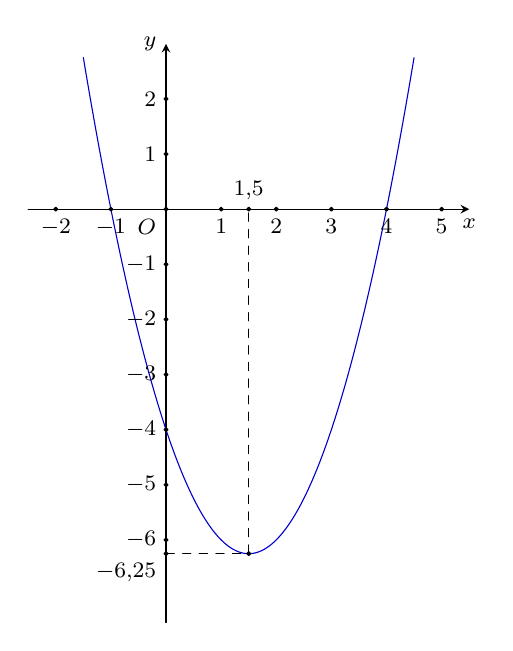
\begin{tikzpicture}[scale=0.7, font=\footnotesize, line join=round, line cap=round, >=stealth]
			\draw [->] (-2.5,0)--(5.5,0) node[below]{$x$};
			\draw [->] (0,-7.5)--(0,3) node[left]{$y$};
			\draw[fill=black] (0,0) circle(1pt) node[below left]{$O$};
			\clip (-2.5,-7.5) rectangle (5.5,3);
			\draw[color=blue!80!black,smooth, samples=300, domain=-1.5:4.5] plot (\x,{(\x)^2-3*(\x)-4});
			\draw[fill=black] (1.5,-6.25) circle(1pt);
			\foreach \i in {-2,-1,1,2,3,4,5} \draw[fill=black] (\i,0) circle(1pt) node[below]{$\i$};
			\foreach \j in {-6,-5,-4,-3,-2,-1,1,2} \draw[fill=black] (0,\j) circle(1pt) node[left]{$\j$};
			\draw[fill=black] (1.5,0) circle(1pt) node[above]{$1{,}5$};
			\draw[fill=black] (0,-6.25) circle(1pt) node[below left]{$-6{,}25$};
			\draw[dashed] (0,-6.25)-|(1.5,0);
		\end{tikzpicture}
	\end{center}
	Gọi $M$ là giá trị nhỏ nhất của hàm số. Hãy xác định giá trị của biểu thức 
	\begin{center}
		$T=\dfrac{2\, 024 \cdot f(-1)+2\, 025 \cdot f(3)+f(0)}{2\, 026 \cdot M}$ (làm tròn đến hàng phần trăm).
	\end{center}
	\shortans{$0{,}64$}
	\loigiai{
		Dựa vào đồ thị ta thấy $f(-1)=0$, $f(0)=-4$ và giá trị nhỏ nhất của hàm số là $M=-6{,}25$.\\
		Vì $x=1{,}5$ là trục đối xứng của đồ thị hàm số, mà $x=0, x=3$ đối xứng nhau qua trục nên $f(0)=f(3) \Rightarrow f(3)=-4$.\\
		Vậy $T=\dfrac{2\, 024 \cdot 0+2\, 025 \cdot(-4)+(-4)}{2\, 026 .(-6{,}25)}=\dfrac{4}{6{,}25}=0{,}64$.}
\end{ex}
\begin{ex}
	Lớp $10A1$ có $45$ học sinh chuẩn bị cho hội diễn văn nghệ chào mừng ngày nhà giáo Việt Nam
	20/11. Trong danh sách đăng kí tham gia tiết mục nhảy Flashmob và tiết mục hát, có $35$ học sinh
	tham gia tiết mục nhảy Flashmob, $10$ học sinh tham gia cả hai tiết mục. Hỏi có bao nhiêu học
	sinh trong lớp tham gia tiết mục hát? Biết rằng lớp 1 có$10A1$ bạn An, Bình, Chi, Danh bị ốm nên không tham gia tiết mục nào, còn lại bạn nào cũng phải tham gia ít nhất 1 trong
	2 tiết mục .
	\shortans{$16$}
	\loigiai{
		Vì có $4$ học sinh không tham gia nên có ít nhất $45-4=41$ học sinh tham gia ít nhất một môn.\\
		Vì có $35$ học sinh tham gia tiết mục nhảy nên có $41-35=6$ học sinh chỉ tham gia tiết mục hát mà không tham gia tiết mục nhảy. Như vậy có $6+10=16$ học sinh tham gia tiết mục hát.\\
		Ta có thể sử dụng công thức $|A \cup B|=|A|+|B|-|A \cap B|$ với $A$ là tập hợp các học sinh tham gia nhảy, $B$ là tập hợp các học sinh tham gia hát và $A \cap B$ là tập hợp các học sinh vừa nhảy vừa hát. Vậy nên $|B|=|A \cup B|+|A \cap B|-|A|=41+10-35=16$.
		
	}
\end{ex}
\begin{ex}%[0D3V2-6]%[CTST - Lớp 10 - Ôn tập giữa học kì 1 - Đề 3]%[Nguyễn Hoài Nam]
	Nữ vận động viên bóng chuyền đánh một quả bóng sang phần sân đối phương với vị trí ban đầu
	từ độ cao $4$ ft (là khoảng cách từ điểm bóng chạm tay đến mặt sân). Tính từ thời điểm quả bóng
	được đánh đi, sau $0{,}5$ s quả bóng ở độ cao $10$ ft và sau $1$ s quả bóng ở độ cao $8$ ft. Biết biểu thức	tính độ cao của quả bóng so với mặt sân $h(t)$ theo thời gian $t$ là một hàm số bậc hai. Hỏi đối
	phương có bao nhiêu giây tính từ lúc quả bóng được đánh đi để chạy đến cứu quả bóng trước khi	nó chạm mặt sân, kết quả lấy đến hàng phần trăm? (ft: feet, là đơn vị đo độ dài, $1$ ft=$30{,}48$ cm).
	\shortans{$1{,}43$}
	\loigiai{
		\begin{center}
			\begin{tikzpicture}[scale=1, font=\footnotesize, line join=round, line cap=round, >=stealth]
				\draw[->] (-2.1,0)--(5,0) node[below left] {$t$};
				\draw[->] (0,-1)--(0,6) node[below right] {$h$};
				\draw (0,0) node [above left] {$O$};
				\draw[fill=black] (3,0) circle(1pt) node[below]{$M$};
				\draw[fill=black] (0,2) circle(1pt) node[below right]{$A$};
				\draw[fill=black] (1,5) circle(1pt) node[above]{$B$};
				\draw[fill=black] (2,4.333) circle(1pt) node[above right]{$C$};
				\draw[fill=black] (2,0) circle(1pt) node[below]{$1$};
				\draw[fill=black] (0,2) circle(1pt) node[above left]{$4$};
				\draw[fill=black] (1,0) circle(1pt) node[below]{$\dfrac{1}{2}$};
				\draw[fill=black] (0,5) circle(1pt) node[above left]{$10$};
				\draw[fill=black] (0,4.333) circle(1pt) node[above left]{$8$};
				\draw[dashed](1,0)--(1,5)--(0,5);\draw[dashed](2,0)--(2,4.333)--(0,4.333);
				\begin{scope}
					\clip (0,0) rectangle (4,6);
					\draw[samples=200,domain=-4:4,smooth,variable=\t] plot (\t,{-1.83*(\t)^2+4.83*(\t)+2})node[above right]{$C$};
				\end{scope}
			\end{tikzpicture}
			
		\end{center}
		Dựng hệ hệ tọa độ $Oth$ như hình vẽ, với gốc tọa độ $O$ trùng với vị trí là hình chiếu của quả bóng trên mặt sân khi nó được đánh đi.
		Gọi parabol $(P) \colon h(t)=at^2+bt+c$.\\
		Vị trí ban đầu có độ cao $4$ ft nên $A(0;4) \in (P) \Leftrightarrow c=4 \quad (1)$.\\
		Ta có $0{,}5$ giây sau khi được đánh đi quả bóng ở độ cao $10$ ft nên $B\left(\dfrac{1}{2};10\right) \in (P)$ \\
		$\Leftrightarrow \dfrac{1}{4}a+\dfrac{1}{2}b+c=10 \quad (2)$.\\
		Ta có $1$ giây sau khi được đánh đi quả bóng ở độ cao $8$ ft nên $C(1;8)\in (P)$\\
		$ \Leftrightarrow a+b+c=8 \quad (3)$.\\
		Từ $(1)$, $(2)$, $(3)$ Ta có hệ phương trình 
		$\heva{&c=4\\&\dfrac{1}{4}a+\dfrac{1}{2}b+c=10\\&a+b+c=8} \Leftrightarrow \heva{&a=-16\\&b=20\\&c=4.}$\\
		Vậy $h(t)=-16t^2+20t+4$.\\
		Khi quả bóng chạm đất thì $h(t)=0 \Leftrightarrow -16t^2+20t+4=0 \Leftrightarrow \hoac{&t=\dfrac{5+\sqrt{41}}{8}\approx 1{,}3\\&t=\dfrac{5+\sqrt{41}}{8} \approx -0{,}18.}$\\
		Vậy đối phương có $1{,}43$ giây để cứu bóng trước khi quả bóng chạm mặt sân.
	}
\end{ex}

\Closesolutionfile{ans}

\indapan{6}{ans-KQ}